\subsection{Expressions derived from \( \pi \):}
One may easily derive the average number of individuals that are at any given state 
using \( pi \). 
The average number of individuals in state \( i \) can be calculated by multiplying 
the number of individuals that are present in state \( i \) with the probability 
of being at that particular state (i.e \(\pi_i (u_i + v_i)\)). 
Using this logic it is possible to calculate any performance measures that are related 
to the mean number of individuals in the system.


Average number of people in the system: 
\begin{equation}
    L = \sum_{i=1}^{|\pi|} \pi_i (u_i + v_i)
\end{equation} 

Average number of people in the service centre: 
\begin{equation}
    L_H = \sum_{i=1}^{|\pi|} \pi_i v_i
\end{equation}

Average number of people in the buffer centre:
\begin{equation}
    L_A = \sum_{i=1}^{|\pi|} \pi_i u_i
\end{equation}

Consequently getting the performance measures that are related to the duration of 
time is not as straightforward. 
Such performance measures are the mean waiting time in the system and the mean time 
blocked in the system. 
Under the scope of this study three approaches have been considered to calculate these 
performance measures; a direct approach, a recursive algorithm and consequently a
closed-form formula.

The research question that needs to be answered here is: ``When a class 1/2 
individuals enters the system, what is the expected time that they will have to 
wait?''. 
In order to formulate the answer to that question one needs to consider all possible 
scenarios of what state the system can be in when an individual arrives. 
Furthermore, different formulas arises for class 1 individuals 
and a different one for class 2 individuals.

\subsection{Mean waiting time} 
\subsubsection{Recursive formula for mean waiting time of class 1 individuals}
\label{sec:recursive-waiting-time-others}

To calculate the mean waiting time of class 1 individuals one must first identify 
the set of states \((u, v)\) that will imply that a wait will occur. 
For this particular Markov chain, this points to all states that satisfy \(v > C\) 
i.e. all states where the number of individuals in the service centre exceed the 
number of servers. 
The set of such states is defined as \textit{waiting states} and can be denoted 
as a subset of all the states, where:

\begin{equation} \label{eq:waiting_states}
    S_w = \{(u, v) \in S \; | \; v > C \}    
\end{equation}

Additionally, there are certain states in the model where arrivals cannot occur. 
A class 1 individual cannot arrive whenever the model is at any state 
\((u, N)\) 
for all \(u\) where \(N\) is the system capacity. 
Therefore the set of all such states that an arrival may occur are defined as 
\textit{accepting states} and are denoted as:

\begin{equation}\label{eq:accepting_states_others}
    S_A^{(1)} = \{(u, v) \in S \; | \; v < N \}
\end{equation}



Moreover, another element that needs to be considered is the expected waiting time 
in each state \( c(u,v) \), otherwise known as sojourn time. 
In order to do so a variation of the Markov model has to be considered where when 
the individual arrives at any of the states of the model no more arrivals can 
occur after that. 


\begin{figure}[h]
    \centering
    \begin{tikzpicture}[-, node distance = 1.4cm, auto]

        \tikzmath{
            let \minsz = 1.8cm;
        }

        \node[draw=none, minimum size=\minsz] (one) {};
        \node[state, minimum size=\minsz, right=of one] (two) {(0,T-1)};
        \node[state, minimum size=\minsz, right=of two] (three) {(0,T)};
        \node[state, minimum size=\minsz, right=of three] (four) {(0,T+1)};
        \node[draw=none, minimum size=\minsz, right=of four] (five) {};

        \node[state, draw=red, line width=0.5mm, minimum size=\minsz, 
        below=of three] (three_one) {(1,T)};
        \node[state, draw=red, line width=0.5mm, minimum size=\minsz, 
        below=of three_one] (three_two) {(2,T)};
        \node[state, minimum size=\minsz, below=of four] (four_one) {(1,T+1)};
        \node[state, minimum size=\minsz, below=of four_one] (four_two) {(2,T+1)};
        \node[draw=none, minimum size=\minsz, right=of four_one] (five_one) {};
        \node[draw=none, minimum size=\minsz, right=of four_two] (five_two) {};
        \node[draw=none, minimum size=\minsz, below=of three_two] (three_three) {};

        \draw[every loop]
            (two) edge node {\((T-1) \mu\)} (one)
            (three) edge node {\(T \mu\)} (two)
            (four) edge node {\((T+1) \mu\)} (three)
            (five) edge node {\((T+1) \mu\)} (four)
            (three_one) edge node {\(T \mu\)} (three)

            (four_one) edge node {\((T+1) \mu\)} (three_one)
            (five_one) edge node {\((T+1) \mu\)} (four_one)
            (three_two) edge node {\(T \mu\)} (three_one)
            (three_three) edge node {\(T \mu\)} (three_two)
            (four_two) edge node {\((T+1) \mu\)} (three_two)
            (five_two) edge node {\((T+1) \mu\)} (four_two)
            ;       
        
        \draw[->, red, ultra thick] (three_two) edge node {} (two);
        \draw[->, red, ultra thick] (three_one) edge node {} (two);
    \end{tikzpicture}
    \caption{Markov chain - ignoring any arrivals} 
    \label{other_patients_trip}
\end{figure}

As illustrated in figure \ref{other_patients_trip} a class 1 individual, 
when in the threshold column, only visits one of the nodes since they are not 
affected by class 2 individuals. 
Thus, one may acquire the desired time by calculating the inverse of the sum of 
the out-flow rate of that state. 
Since we are ignoring arrivals though the only way to exit the state will only be 
via a service. 
In essence this notion can be expressed as:

\begin{equation} \label{eq:sojourn_others}
    c^{(1)}(u,v) = 
    \begin{cases}
        0, & \textbf{if } u > 0 \textbf{ and } v = T \\
        \frac{1}{\text{min}(v,C)\mu}, & \textbf{otherwise}
    \end{cases}
\end{equation}

Note that whenever any class 1 individual is at a state \((u,v)\) where 
\(u > 0\) 
and \(v = T\) (i.e. all states \((1,T), (2,T) \dots, (M,T)\)) the sojourn time is 
set to \(0\). 
This is done to capture the trip thorough the Markov chain from the perspective 
of class 1 individuals. 
Meaning that they will visit all states of the threshold column but only the one 
in the first row will return a non-zero sojourn time.

Now, using the above equations, and considering all sates that belong in \(S_w\) 
the following recursive formula can be used to get the mean waiting time spent in 
each state in the Markov model. 
For class 1 individuals, whenever the model is at state \( (u,v) \), any 
incoming 
individual will proceed to arrive at state \( (u, v+1) \). 
individuals will then proceed to visit all other states until they reach one which 
has less than \(C\) servers occupied (i.e. until a server becomes available). 
The formula goes through all states from right to left recursively and adds the 
sojourn times of all these states together until it reaches a state that is not 
in the set of waiting states. 
Thus, the expected waiting time of a class 1 individual when they arrive at 
state \( (u,v) \) can be given by:

\begin{equation} \label{eq:waiting-time-at-each-state-other}
    w^{(1)}(u,v) = 
    \begin{cases} 
        0, \hspace{4.85cm} & \textbf{if } (u,v) \notin S_w \\
        c^{(1)}(u,v) + w^{(1)}(u-1, v), & \textbf{if } u > 0 \textbf{ and } v = T \\
        c^{(1)}(u,v) + w^{(1)}(u, v-1), & \textbf{otherwise}
    \end{cases}
\end{equation}

Finally, the overall mean waiting time can be calculated by summing over all expected 
waiting times of accepting states multiplied by the probability of being at that 
state and dividing by the probability of being in any accepting state.

\begin{equation} \label{eq:recursive-waiting-time-others}
    W^{(1)} = \frac{\sum_{(u,v) \in S_A^{(1)}} w^{(1)}(u,v) 
    \pi_{(u,v)}}{\sum_{(u,v) \in S_A^{(1)}} \pi_{(u,v)}}
\end{equation}



\subsubsection{Recursive formula for mean waiting time of 
class 2 individuals} \label{sec:recursive-waiting-time-ambulance}

Equivalently the mean waiting time for class 2 individuals can be calculated 
in a similar manner. 
The set of waiting states is the same as before but there is a slight modification 
in the set of accepting states.

\[
    S_w = \{(u, v) \in S \; | \; v > C \}    
\]

\begin{equation}\label{eq:accepting_states_ambulance}
    S_A^{(2)}=
    \begin{cases}
        \{(u, v) \in S \; | \; u < M \} & \textbf{if } T \leq N\\
        \{(u, v) \in S \; | \; v < N \} & \textbf{otherwise}
    \end{cases}
\end{equation}

The set of accepting states is modified in such a way such that a class 2 
individual cannot arrive in the model when the model is at any state \((M, v)\) 
for 
all \(v \geq T\) where \(M\) is the buffer centre capacity and \(T\) is the threshold. 
An odd situation here is when the threshold is set to a very high number that is 
more than the actual system capacity. 
In such cases the set of accepting states is defined in the same way as the 
class 1 individuals case (\ref{eq:accepting_states_others}). 
That is because whenever \(T > N\) no class 2 individual will ever be blocked in 
the model 
(since that threshold can never be reached) and thus the last accepting state of 
the model will be state \( (0,N-1)\). 

Now just like in the class 1 individuals case the sojourn time is needed. 
For class 2 individuals whenever individuals are at any row apart from the 
first one they automatically get a wait time of \(0\) since they are essentially 
blocked.

\begin{equation} \label{eq:sojourn_ambulance}
    c^{(2)}(u,v) = 
    \begin{cases}
        0, & \textbf{if } u > 0 \\
        \frac{1}{\text{min}(v,C)\mu}, & \textbf{otherwise}
    \end{cases}
\end{equation}

Finally, the recursive formula and the mean waiting time equation are identical 
to the ones described above with the exception that they now use \(c^{(2)}(u,v)\) 
instead of \(c^{(1)}(u,v)\).
\begin{equation} \label{eq:waiting-time-at-each-state-ambulance}
    w^{(2)}(u,v) = 
    \begin{cases} 
        0, \hspace{4.85cm} & \textbf{if } (u,v) \notin S_w \\
        c^{(2)}(u,v) + w^{(2)}(u-1, v), & \textbf{if } u > 0 \textbf{ and } v = T \\
        c^{(2)}(u,v) + w^{(2)}(u, v-1), & \textbf{otherwise}
    \end{cases}
\end{equation}

\begin{equation}\label{eq:recursive-waiting-time-ambulance}
    W^{(2)} = \frac{\sum_{(u,v) \in S_A^{(2)}} w^{(2)}(u,v) \pi_{(u,v)}}
    {\sum_{(u,v) \in S_A^{(2)}} \pi_{(u,v)}}
\end{equation}

\subsubsection{Mean Waiting Time - Closed-form}
Upon closer inspection of the recursive formula a more compact formula can arise. 
The equivalent closed-form formula eliminates the need for recursion and thus makes 
the computation of waiting times much more efficient. 
Just like in the recursive part there are two formulas; one for \textit{class 1} 
and one for class 2 individuals. 
The formulas are given by:

\begin{equation} \label{eq:closed_form_waiting_others}
    W^{(1)} = \frac{\sum_{\substack{(u,v) \, \in S_A^{(1)} \\ v \geq C}} 
    \frac{1}{C \mu} \times (v-C+1) \times \pi(u,v)}{\sum_{(u,v) \, 
    \in S_A^{(1)}} \pi(u,v)}
\end{equation}
    
\begin{equation}\label{eq:closed_form_waiting_ambulance}
    W^{(2)} = \frac{\sum_{\substack{(u,v) \, \in S_A^{(2)} \\ min(v,T) \geq C}} 
    \frac{1}{C \mu} \times (\min(v+1,T)-C) \times \pi(u,v)}{\sum_{(u,v) \, 
    \in S_A^{(2)}} \pi(u,v)}
\end{equation}

Note here that the summation, in both equations \ref{eq:closed_form_waiting_others} 
and \ref{eq:closed_form_waiting_ambulance}, goes through all states in the set of 
accepting 
states of either class 1 or class 2 individuals respectively, where a wait 
incurs. 
In equation \ref{eq:closed_form_waiting_others} that includes all states \((u,v)\) 
in the set of accepting states of class 1 individuals such that \( v \geq C\); i.e. 
whenever an arrival occurs and the system is at a state where the number of individuals 
in the system is more than or equal to $C$. 
Consequently, for the states that are included in the summation the expression 
\( v-C+1 \) indicates the amount of people in service one would have to wait for 
upon arrival at the hospital.

Additionally, the minimisation function in equation 
\ref{eq:closed_form_waiting_ambulance} 
ensures that when a class 2 individual arrives at any state 
that is greater than the predetermined threshold, the wait that the individual will 
have to endure remains the same. 
In essence, the expression \(\min(v+1,T) - C\) returns the number of people in line 
in front of a particular individual upon arrival.


\subsubsection{Overall Waiting Time}

Consequently, the overall waiting time should can be estimated by a linear combination 
of the waiting times of class 1 and class 2 individuals. 
The overall waiting time can be then given by the following equation where \(c_1\) 
and \(c_2\) are the coefficients of each individual's type waiting time:

\begin{equation}\label{overall_waiting_time_coeff}
    W = c_1 W^{(1)} + c_2 W^{(2)}
\end{equation}

The two coefficients represent the proportion of individuals of each type that 
traversed through the model. 
Theoretically, getting these percentages should be as simple as looking at the arrival 
rates of each type but in practise if the service centre or the buffer centre 
is full, some individuals may be lost to the system. 
Thus, one should account for the probability that an individual is lost to the system. 
This probability can be easily calculated by using the two sets of accepting states 
\(S_A^{(2)}\) and \(S_A^{(1)}\) defined earlier in equations 
\ref{eq:accepting_states_others} 
and \ref{eq:accepting_states_ambulance}. 
Let us define here the probability, for either class type, that an individual 
is not lost in the system by:

\begin{equation*}
    P(L'_1) = \sum_{(u,v) \, \in S_A^{(1)}} \pi(u,v) \hspace{2cm}
    P(L'_2) = \sum_{(u,v) \, \in S_A^{(2)}} \pi(u,v)
\end{equation*}

Having defined these probabilities one may combine them with the arrival rates of 
each class type in such a way to get the expected proportions of class 1 and 
class 2 individuals in the model. 
Thus, by using these values as the coefficient of equation 
\ref{overall_waiting_time_coeff} 
the resultant equation can be used to get the overall waiting time. 
Note here that the equation below gets the overall waiting time for both the recursive 
and the closed-form formula.

\begin{equation}\label{overall_waiting_time}
    W = \frac{\lambda_1 P(L'_1)}{\lambda_2 P(L'_2) + \lambda_1 P(L'_1)} W^{(1)} + 
    \frac{\lambda_2 P(L'_2)}{\lambda_2 P(L'_2) + \lambda_1 P(L'_1)} W^{(2)}
\end{equation}


% \newpage
% Mean waiting time in the hospital:
% \begin{equation}
%     W_q = \sum_{i=1}^{|\pi|} \frac{\text{max}(v_i - C, 0) \; \pi_i}{\sum_{\substack{j=1 \\ i \neq j}}^{|\pi|} q_{i j}}
% \end{equation}

% \begin{equation}
%     W_q = \sum_{i=1}^{|\pi|} \pi_i \frac{v_i - c}{v_i \mu}, \quad v_i > c
% \end{equation}


\subsection{Mean blocking time}

\subsubsection{Direct approach for mean blocking time}

Unlike the waiting time, the blocking time is only calculated for class 2 individuals.  
That is because class 1 individuals cannot be blocked. 
Thus, one only needs to consider the pathway of class 2 individuals to get the 
mean blocking time of the system. 
Blocking occurs at states \((u,v)\) where \(u > 0 \). 
Thus, the set of blocking states can be defined as:

\begin{equation*}
    S_b = \{(u,v) \in S \; | \; u > 0\}
\end{equation*}
 
In order to not consider individuals that will be lost to the system, the set of 
accepting states needs to be taken into account. As defined in section 
\ref{sec:recursive-waiting-time-ambulance},
the set of accepting states is given by (\ref{eq:accepting_states_ambulance}):

\begin{equation*}
    S_A^{(2)}=
    \begin{cases}
        \{(u, v) \in S \; | \; u < M \} & \textbf{if } T \leq N\\
        \{(u, v) \in S \; | \; v < N \} & \textbf{otherwise}
    \end{cases}
\end{equation*}

For the waiting time formula in sections \ref{sec:recursive-waiting-time-others}
and \ref{sec:recursive-waiting-time-ambulance}
the mean sojourn time for each state was considered,
ignoring any arrivals. Here, the same approach is used but ignoring only class 2
arrivals. That is because for the waiting time formula, once an individual enters 
the service centre (i.e. starts waiting) any individual arriving after them will 
not affect their
pathway. That is not the case for blocking time. When a class 2 individual is 
blocked, 
any class 1 individual that arrives will cause the blocked individual to remain 
blocked for more time. Therefore, class 1 arrivals are considered here:

\begin{equation}\label{eq:time_in_state_blocking_time}
    c(u,v) = 
    \begin{cases}
        \frac{1}{\min(v,C) \mu}, & \text{if } v = C\\
        \frac{1}{\min(v,C) \mu + \lambda_1}, & \text{otherwise}
    \end{cases}
\end{equation}
 
In equation \ref{eq:time_in_state_blocking_time}, both service completions and 
class 1 arrivals are considered. 
Thus, from a blocked individual's perspective whenever the system moves from one 
state \((u,v)\)
to another state it can either:

\begin{itemize}
    \item be because of a service being completed: we will denote the probability 
    of this happening by \(p_s(u,v)\). 
    \item be because of an arrival of an individual of class 1: denoting such 
    probability by \(p_o(u,v)\).
\end{itemize}
The probabilities are given by:

\begin{equation*}
    p_s(u,v) = \frac{\min(v,C)\mu}{\lambda_1 + \min(v,C)\mu}, \qquad
    p_o(u,v) = \frac{\lambda_1}{\lambda_1 + \min(v,C)\mu}
\end{equation*}


Having defined \(c(u,v)\) and \(S_b\) a formula for the blocking time that is
expected to occur at each state can be given by:

\begin{equation}\label{eq:blocking-time-at-each-state}
    b(u,v) = 
    \begin{cases} 
        0, & \textbf{if } (u,v) \notin S_b \\
        c(u,v) + b(u - 1, v), & \textbf{if } v = N = T\\
        c(u,v) + b(u, v-1), & \textbf{if } v = N \neq T \\
        c(u,v) + p_s(u,v) b(u-1, v) + p_o(u,v) b(u, v+1), & \textbf{if } u > 0 
        \textbf{ and } v = T \\
        c(u,v) + p_s(u,v) b(u, v-1) + p_o(u,v) b(u, v+1), & \textbf{otherwise} \\
    \end{cases}
\end{equation}

Unlike equations (\ref{eq:waiting-time-at-each-state-other}) and 
(\ref{eq:waiting-time-at-each-state-ambulance}), equation 
(\ref{eq:blocking-time-at-each-state}) will not be solved recursively. 
A direct approach will be used to solve this equation here. 
By enumerating all equations of (\ref{eq:blocking-time-at-each-state}) for all 
states \((u,v)\) that belong in \(S_b\) 
a system of linear equations arises where the unknown variables are all the \(b(u,v)\)
terms.
For instance, let us consider a Markov model where \(C=2, T=3, N=6, M=2\). 
The Markov model is shown in Figure \ref{fig:example-algeb-blocking}
and the equivalent equations are 
(\ref{eq:first_eq_of_blocking_example})-(\ref{eq:last_eq_of_blocking_example}).
The equations considered here are only the ones that correspond to the blocking 
states.

\begin{multicols*}{2}
    \begin{figure}[H]
        \scalebox{0.50}{\section{Figures that might be useful}
\begin{figure}[h]
    \centering
    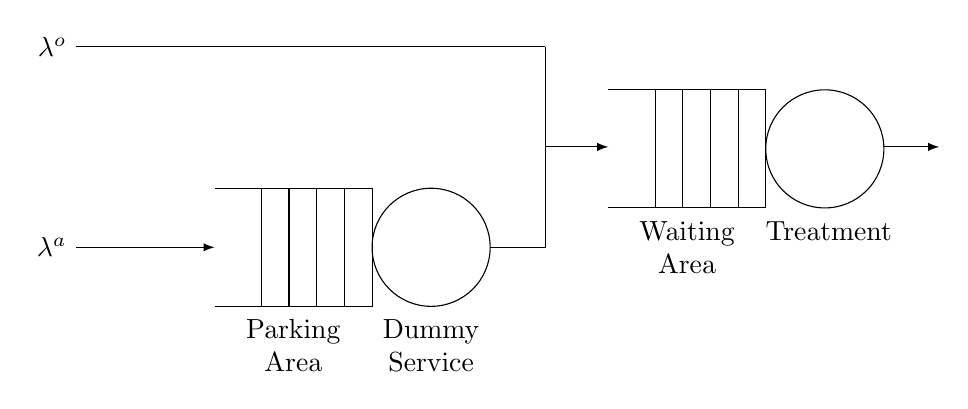
\begin{tikzpicture}[>=latex]
        % the rectangle with vertical rules (Queue 1)
        \draw (0,0) -- ++(2cm,0) -- ++(0,-1.5cm) -- ++(-2cm,0);
        \foreach \i in {1,...,4}
        \draw (2cm-\i*10pt,0) -- +(0,-1.5cm);
        
        % the circle (Queue 1)
        \draw (2.75,-0.75cm) circle [radius=0.75cm];

        % the rectangle with vertical rules (Queue 2)
        \draw (5,1.25) -- ++(2cm,0) -- ++(0,-1.5cm) -- ++(-2cm,0);
        \foreach \i in {1,...,4}
        \draw (7cm-\i*10pt,1.25) -- +(0,-1.5cm);

        % the circle (Queue 2)
        \draw (7.75,0.5) circle [radius=0.75cm];

        % the arrows and labels (Queue 1+2)
        \draw[-] (3.5,-0.75) -- +(20pt,0);
        \draw[<-] (0,-0.75) -- +(-50pt,0) node[left] {\( \lambda^a \)};
        \draw[->] (8.5,0.525) -- +(20pt,0);
        \node[align=center] at (1cm,-2cm) {Parking \\ Area};
        \node[align=center] at (2.75cm,-2cm) {Dummy \\ Service};
        \node[align=center] at (6cm,-0.75cm) {Waiting \\ Area};
        \node[align=center] at (7.8cm,-0.75cm) {Treatment \\ };
        
        \draw (4.2, 1.8) -- +(-169.5pt,0) node[left] {\( \lambda^o \)};
        \draw (4.2, 1.8) -- (4.2, -0.75);
        \draw[->] (4.2, 0.525) -- (5, 0.525);

    \end{tikzpicture}
\end{figure}


\begin{figure}
    \centering
    \begin{tikzpicture}[-, node distance = 1cm, auto, every node/.style={scale=0.5}]

        % Variables
        \tikzmath{
            let \altdist = 1.5cm;
            let \minsz = 1.5cm;
        }

        % First Line
        \node[state, minimum size=1.5cm] (zero) {(0,0)};
        \node[state, minimum size=1.5cm,  right=of zero] (one) {(0,1)};
        \node[draw=none, minimum size=1.5cm, right=of one] (two) {\dots};
        \node[state, minimum size=1.5cm, right=of two] (three) {(0,T)};
        \node[state, node distance = \altdist, minimum size=\minsz, right=of three] (four) {(0,T+1)};
        \node[draw=none, node distance = \altdist, minimum size=\minsz, right=of four] (five) {\dots};
        \node[state, node distance = \altdist, minimum size=\minsz, right=of five] (six) {(0,C)};
        \node[draw=none, minimum size=\minsz, right=of six] (seven) {\dots};

        % Second Line
        \node[state, minimum size=\minsz, below=of three] (three_one) {(1,T)};
        \node[state, minimum size=\minsz, below=of four] (four_one) {(1,T+1)};
        \node[draw=none, minimum size=\minsz, below=of five] (five_one) {\dots};
        \node[state, node distance = \altdist, minimum size=\minsz, right=of five_one] (six_one) {(1,C)};
        \node[draw=none, minimum size=\minsz, right=of six_one] (seven_one) {\dots};

        % Third Line
        \node[state, minimum size=\minsz, below=of three_one] (three_two) {(2,T)};
        \node[state, minimum size=\minsz, below=of four_one] (four_two) {(2,T+1)};
        \node[draw=none, minimum size=\minsz, below=of five_one] (five_two) {\dots};
        \node[state, node distance = \altdist, minimum size=\minsz, right=of five_two] (six_two) {(2,C)};
        \node[draw=none, minimum size=\minsz, right=of six_two] (seven_two) {\dots};

        % Fourth line
        \node[draw=none, minimum size=\minsz, below=of three_two] (three_three) {\vdots};
        \node[draw=none, minimum size=\minsz, below=of four_two] (four_three) {\vdots};
        \node[draw=none, minimum size=\minsz, below=of five_two] (five_three) {};
        \node[draw=none, node distance = \altdist, minimum size=\minsz, right=of five_three] (six_three) {\vdots};

        \draw[every loop]
            % First Horizontal Edges
            (zero) edge[bend left] node {\( \Lambda \)} (one)
            (one) edge[bend left] node [above] {\( \mu \)} (zero)
            (one) edge[bend left] node {\( \Lambda \)} (two)
            (two) edge[bend left] node [above] {\( 2 \mu \)} (one)
            (two) edge[bend left] node {\( \Lambda \)} (three)
            (three) edge[bend left] node [above] {\( T \mu \)} (two)
            (three) edge[bend left] node {\( \lambda^o \)} (four)
            (four) edge[bend left] node [above] {\( (T+1) \mu \)} (three)
            (four) edge[bend left] node {\( \lambda^o \)} (five)
            (five) edge[bend left] node [above] {\( (T+2) \mu \)} (four)
            (five) edge[bend left] node {\( \lambda^o \)} (six)
            (six) edge[bend left] node [above] {\( C\mu \)} (five)
            (six) edge[bend left] node {\( \lambda^o \)} (seven)
            (seven) edge[bend left] node [above] {\( C\mu \)} (six)

            % Second Horizontal Edges
            (three_one) edge[bend left] node {\( \lambda^o \)} (four_one)
            (four_one) edge[bend left] node [above] {\( (T+1) \mu \)} (three_one)
            (four_one) edge[bend left] node {\( \lambda^o \)} (five_one)
            (five_one) edge[bend left] node [above] {\( (T+2) \mu \)} (four_one)
            (five_one) edge[bend left] node {\( \lambda^o \)} (six_one)
            (six_one) edge[bend left] node [above] {\( C\mu \)} (five_one)
            (six_one) edge[bend left] node {\( \lambda^o \)} (seven_one)
            (seven_one) edge[bend left] node [above] {\( C\mu \)} (six_one)

            % Third Horizontal Edges
            (three_two) edge[bend left] node {\( \lambda^o \)} (four_two)
            (four_two) edge[bend left] node [above] {\( (T+1) \mu \)} (three_two)
            (four_two) edge[bend left] node {\( \lambda^o \)} (five_two)
            (five_two) edge[bend left] node [above] {\( (T+2) \mu \)} (four_two)
            (five_two) edge[bend left] node {\( \lambda^o \)} (six_two)
            (six_two) edge[bend left] node [above] {\( C\mu \)} (five_two)
            (six_two) edge[bend left] node {\( \lambda^o \)} (seven_two)
            (seven_two) edge[bend left] node [above] {\( C\mu \)} (six_two)

            % First Vertical Edges
            (three) edge[bend left] node {\( \lambda^A \)} (three_one)
            (three_one) edge[bend left] node {\( T \mu \)} (three)
            (three_one) edge[bend left] node {\( \lambda^A \)} (three_two)
            (three_two) edge[bend left] node {\( T\mu \)} (three_one)
            (three_two) edge[bend left] node {\( \lambda^A \)} (three_three)
            (three_three) edge[bend left] node {\( T\mu \)} (three_two)

            % Second Vertical Edges
            (four) edge node {\( \lambda^A \)} (four_one)
            (four_one) edge node {\( \lambda^A \)} (four_two)
            (four_two) edge node {\( \lambda^A \)} (four_three)

            %Third Vertical Edges
            (six) edge node {\( \lambda^A \)} (six_one)
            (six_one) edge node {\( \lambda^A \)} (six_two)
            (six_two) edge node {\( \lambda^A \)} (six_three)
            ;       
    \end{tikzpicture}
    \caption{Markov chains} 
    \label{Markov_2}
\end{figure}



\begin{figure}
    \centering
    \begin{tikzpicture}[-, node distance = 1cm, auto, every node/.style={scale=0.4}]

        % Variables
        \tikzmath{
            let \altdist = 1cm;
            let \minsz = 1.5cm;
        }

        % First Line
        \node[state, minimum size=1.5cm] (zero) {(0,0)};
        \node[state, minimum size=1.5cm,  right=of zero] (one) {(0,1)};
        \node[draw=none, minimum size=1.5cm, right=of one] (two) {\dots};
        \node[state, minimum size=1.5cm, right=of two] (three) {(0,T)};
        \node[state, node distance = \altdist, minimum size=\minsz, right=of three] (four) {(0,T+1)};
        \node[draw=none, minimum size=\minsz, right=of four] (five) {\dots};
        \node[draw=none, minimum size=\minsz, right=of five] (six) {\vdots};
        \node[draw=none, minimum size=\minsz, right=of six] (seven) {\dots};
        \node[state, minimum size=\minsz, right=of seven] (eight) {(0,C)};
        \node[draw=none, minimum size=\minsz, right=of eight] (nine) {\dots};


        % Second Line
        \node[state, minimum size=\minsz, below=of three] (three_one) {(1,T)};
        \node[state, minimum size=\minsz, below=of four] (four_one) {(1,T+1)};
        \node[draw=none, minimum size=\minsz, below=of five] (five_one) {\dots};
        \node[state, node distance = \altdist, minimum size=\minsz, right=of five_one] (six_one) {\( (u_i, v_i) \)};
        \node[draw=none, minimum size=\minsz, right=of six_one] (seven_one) {\dots};
        \node[state, node distance = \altdist, minimum size=\minsz, right=of seven_one] (eight_one) {(1,C)};
        \node[draw=none, minimum size=\minsz, right=of eight_one] (nine_one) {\dots};
        

        % Third Line
        \node[state, minimum size=\minsz, below=of three_one] (three_two) {(2,T)};
        \node[state, minimum size=\minsz, below=of four_one] (four_two) {(2,T+1)};
        \node[draw=none, minimum size=\minsz, below=of five_one] (five_two) {\dots};
        \node[draw=none, node distance = \altdist, minimum size=\minsz, right=of five_two] (six_two) {\vdots};
        \node[draw=none, minimum size=\minsz, right=of six_two] (seven_two) {\dots};
        \node[state, node distance = \altdist, minimum size=\minsz, right=of seven_two] (eight_two) {(2,C)};
        \node[draw=none, minimum size=\minsz, right=of eight_two] (nine_two) {\dots};

        % Fourth line
        \node[draw=none, minimum size=\minsz, below=of three_two] (three_three) {\vdots};
        \node[draw=none, minimum size=\minsz, below=of four_two] (four_three) {\vdots};
        \node[draw=none, minimum size=\minsz, below=of five_two] (five_three) {};
        \node[draw=none, node distance = \altdist, minimum size=\minsz, right=of five_three] (six_three) {};
        \node[draw=none, node distance = \altdist, minimum size=\minsz, below=of eight_two] (eight_three) {\vdots};


        \draw[every loop]
            % First Horizontal Edges
            (zero) edge[bend left] node {\( \Lambda \)} (one)
            (one) edge[bend left] node {\( \mu \)} (zero)
            (one) edge[bend left] node {\( \Lambda \)} (two)
            (two) edge[bend left] node {\( 2 \mu \)} (one)
            (two) edge[bend left] node {\( \Lambda \)} (three)
            (three) edge[bend left] node {\( T \mu \)} (two)
            (three) edge[bend left] node {\( \lambda^o \)} (four)
            (four) edge[bend left] node {\( (T+1) \mu \)} (three)
            (four) edge[bend left] node {\( \lambda^o \)} (five)
            (five) edge[bend left] node {\( (T+2) \mu \)} (four)
            % (five) edge[bend left] node {\( \lambda^o \)} (six)
            % (six) edge[bend left] node [above] {\( C\mu \)} (five)
            % (six) edge[bend left] node {\( \lambda^o \)} (seven)
            % (seven) edge[bend left] node [above] {\( C\mu \)} (six)
            (seven) edge[bend left] node {\( \lambda^o \)} (eight)
            (eight) edge[bend left] node {\( C\mu \)} (seven)
            (eight) edge[bend left] node {\( \lambda^o \)} (nine)
            (nine) edge[bend left] node {\( C\mu \)} (eight)

            % Second Horizontal Edges
            (three_one) edge[bend left] node {\(\lambda^o\)} (four_one)
            (four_one) edge[bend left] node {\( (T+1) \mu \)} (three_one)
            (four_one) edge[bend left] node {\( \lambda^o \)} (five_one)
            (five_one) edge[bend left] node {\( (T+2) \mu \)} (four_one)
            (five_one) edge[bend left] node {\( \lambda^o \)} (six_one)
            (six_one) edge[bend left] node {\( v_i\mu \)} (five_one)
            (six_one) edge[bend left] node {\( \lambda^o \)} (seven_one)
            (seven_one) edge[bend left] node {\( (v_i+1)\mu \)} (six_one)
            (seven_one) edge[bend left] node {\( \lambda^o \)} (eight_one)
            (eight_one) edge[bend left] node {\( C\mu \)} (seven_one)
            (eight_one) edge[bend left] node {\( \lambda^o \)} (nine_one)
            (nine_one) edge[bend left] node {\( C\mu \)} (eight_one)

            % Third Horizontal Edges
            (three_two) edge[bend left] node {\( \lambda^o \)} (four_two)
            (four_two) edge[bend left] node {\( (T+1) \mu \)} (three_two)
            (four_two) edge[bend left] node {\( \lambda^o \)} (five_two)
            (five_two) edge[bend left] node {\( (T+2) \mu \)} (four_two)
            % (five_two) edge[bend left] node {\( \lambda^o \)} (six_two)
            % (six_two) edge[bend left] node [above] {\( C\mu \)} (five_two)
            % (six_two) edge[bend left] node {\( \lambda^o \)} (seven_two)
            % (seven_two) edge[bend left] node [above] {\( C\mu \)} (six_two)
            (seven_two) edge[bend left] node {\( \lambda^o \)} (eight_two)
            (eight_two) edge[bend left] node {\( C\mu \)} (seven_two)
            (eight_two) edge[bend left] node {\( \lambda^o \)} (nine_two)
            (nine_two) edge[bend left] node {\( C\mu \)} (eight_two)

            % First Vertical Edges
            (three) edge[bend left] node {\( \lambda^A \)} (three_one)
            (three_one) edge[bend left] node {\( T \mu \)} (three)
            (three_one) edge[bend left] node {\( \lambda^A \)} (three_two)
            (three_two) edge[bend left] node {\( T\mu \)} (three_one)
            (three_two) edge[bend left] node {\( \lambda^A \)} (three_three)
            (three_three) edge[bend left] node {\( T\mu \)} (three_two)

            % Second Vertical Edges
            (four) edge node {\( \lambda^A \)} (four_one)
            (four_one) edge node {\( \lambda^A \)} (four_two)
            (four_two) edge node {\( \lambda^A \)} (four_three)

            % Third Vertical Edges
            (six) edge node {\( \lambda^A \)} (six_one)
            (six_one) edge node {\( \lambda^A \)} (six_two)
            % (six_two) edge node {\( \lambda^A \)} (six_three)

            % Fourth Vertical Edges
            (eight) edge node {\( \lambda^A \)} (eight_one)
            (eight_one) edge node {\( \lambda^A \)} (eight_two)
            (eight_two) edge node {\( \lambda^A \)} (eight_three)
            ;       
    \end{tikzpicture}
    \caption{Markov chains} 
    \label{Markov_3}
\end{figure}


\begin{figure}
    \centering
    \begin{tikzpicture}[-, node distance = 0.9cm, auto, every node/.style={scale=0.5}]

        % Variables
        \tikzmath{
            let \initdist = 0.5cm;
            let \altdist = 1.2cm;
            let \minsz = 1.6cm;
            let \leftOne = -0.8;
            let \rightOne = 2.2;
            let \upOne = 0.8;
            let \downOne = -2.2;
            let \leftTwo = 2.25;
            let \rightTwo = 14.2;
            let \upTwo = -2.35;
            let \downTwo = -8.8;
        }

        % % Rectangle for S1
        % \draw[ultra thin, dashed] (\leftOne, \downOne) -- (\leftOne, \upOne);
        % \draw[ultra thin, dashed] (\leftOne, \upOne) -- (\rightOne, \upOne);
        % \draw[ultra thin, dashed] (\rightOne, \upOne) -- node {\Huge{\( \quad S_1 \)}}(\rightOne, \downOne);
        % \draw[ultra thin, dashed] (\rightOne, \downOne) -- (\leftOne, \downOne);

        % % Rectangle for S2
        % \draw[ultra thin, dashed] (\leftTwo, \downTwo) -- node {\Huge{\( S_2 \quad \)}}(\leftTwo, \upTwo);
        % \draw[ultra thin, dashed] (\leftTwo, \upTwo) -- (\rightTwo, \upTwo);
        % \draw[ultra thin, dashed] (\rightTwo, \upTwo) -- (\rightTwo, \downTwo);
        % \draw[ultra thin, dashed] (\rightTwo, \downTwo) -- (\leftTwo, \downTwo);

        % First Line
        \node[state, minimum size=1.5cm] (zero) {(0,0)};
        \node[state, node distance = \initdist, minimum size=\minsz, below right=of zero] (one) {(0,1)};
        \node[draw=none, node distance = \initdist, minimum size=\minsz, below right=of one] (two) {\textbf{\( \ddots \)}};
        \node[state, node distance = \initdist, minimum size=\minsz, below right=of two] (three) {(0,T)};
        \node[state, node distance = \altdist, minimum size=\minsz, right=of three] (four) {(0,T+1)};
        \node[draw=none, node distance = \altdist, minimum size=\minsz, right=of four] (five) {\textbf{\dots}};
        \node[draw=none, minimum size=\minsz, right=of five] (six) {\textbf{\vdots}};
        \node[draw=none, minimum size=\minsz, right=of six] (seven) {\textbf{\dots}};
        \node[state, minimum size=\minsz, right=of seven] (eight) {(0,C)};
        \node[draw=none, minimum size=\minsz, right=of eight] (nine) {\textbf{\dots}};


        % Second Line
        \node[state, minimum size=\minsz, below=of three] (three_one) {(1,T)};
        \node[state, minimum size=\minsz, below=of four] (four_one) {(1,T+1)};
        \node[draw=none, minimum size=\minsz, below=of five] (five_one) {\textbf{\dots}};
        \node[state, minimum size=\minsz, right=of five_one] (six_one) {\( (u_i, v_i) \)};
        \node[draw=none, minimum size=\minsz, right=of six_one] (seven_one) {\textbf{\dots}};
        \node[state, minimum size=\minsz, right=of seven_one] (eight_one) {(1,C)};
        \node[draw=none, minimum size=\minsz, right=of eight_one] (nine_one) {\textbf{\dots}};
        

        % Third Line
        \node[state, minimum size=\minsz, below=of three_one] (three_two) {(2,T)};
        \node[state, minimum size=\minsz, below=of four_one] (four_two) {(2,T+1)};
        \node[draw=none, minimum size=\minsz, below=of five_one] (five_two) {\textbf{\dots}};
        \node[draw=none, minimum size=\minsz, right=of five_two] (six_two) {\textbf{\vdots}};
        \node[draw=none, minimum size=\minsz, right=of six_two] (seven_two) {\textbf{\dots}};
        \node[state, minimum size=\minsz, right=of seven_two] (eight_two) {(2,C)};
        \node[draw=none, minimum size=\minsz, right=of eight_two] (nine_two) {\textbf{\dots}};

        % Fourth line
        \node[draw=none, node distance = \altdist, minimum size=\minsz, below=of three_two] (three_three) {\textbf{\vdots}};
        \node[draw=none, node distance = \altdist, minimum size=\minsz, below=of four_two] (four_three) {\textbf{\vdots}};
        \node[draw=none, node distance = \altdist, minimum size=\minsz, below=of five_two] (five_three) {};
        \node[draw=none, node distance = \altdist, minimum size=\minsz, below=of six_two] (six_three) {};
        \node[draw=none, node distance = \altdist, minimum size=\minsz, below=of eight_two] (eight_three) {\textbf{\vdots}};


        \draw[every loop]
            % First Horizontal Edges
            (zero) edge[bend left] node {\( \Lambda \)} (one)
            (one) edge[bend left] node {\( \mu \)} (zero)
            (one) edge[bend left] node {\( \Lambda \)} (two)
            (two) edge[bend left] node {\( 2 \mu \)} (one)
            (two) edge[bend left] node {\( \Lambda \)} (three)
            (three) edge[bend left] node {\( T \mu \)} (two)
            (three) edge[bend left] node {\( \lambda^o \)} (four)
            (four) edge[bend left] node {\( (T+1) \mu \)} (three)
            (four) edge[bend left] node {\( \lambda^o \)} (five)
            (five) edge[bend left] node {\( (T+2) \mu \)} (four)
            % (five) edge[bend left] node {\( \lambda^o \)} (six)
            % (six) edge[bend left] node [above] {\( C\mu \)} (five)
            % (six) edge[bend left] node {\( \lambda^o \)} (seven)
            % (seven) edge[bend left] node [above] {\( C\mu \)} (six)
            (seven) edge[bend left] node {\( \lambda^o \)} (eight)
            (eight) edge[bend left] node {\( C\mu \)} (seven)
            (eight) edge[bend left] node {\( \lambda^o \)} (nine)
            (nine) edge[bend left] node {\( C\mu \)} (eight)

            % Second Horizontal Edges
            (three_one) edge[bend left] node {\( \lambda^o \)} (four_one)
            (four_one) edge[bend left] node {\( (T+1) \mu \)} (three_one)
            (four_one) edge[bend left] node {\( \lambda^o \)} (five_one)
            (five_one) edge[bend left] node {\( (T+2) \mu \)} (four_one)
            (five_one) edge[bend left] node {\( \lambda^o \)} (six_one)
            (six_one) edge[bend left] node {\( v_i\mu \)} (five_one)
            (six_one) edge[bend left] node {\( \lambda^o \)} (seven_one)
            (seven_one) edge[bend left] node {\( (v_i+1)\mu \)} (six_one)
            (seven_one) edge[bend left] node {\( \lambda^o \)} (eight_one)
            (eight_one) edge[bend left] node {\( C\mu \)} (seven_one)
            (eight_one) edge[bend left] node {\( \lambda^o \)} (nine_one)
            (nine_one) edge[bend left] node {\( C\mu \)} (eight_one)

            % Third Horizontal Edges
            (three_two) edge[bend left] node {\( \lambda^o \)} (four_two)
            (four_two) edge[bend left] node [below] {\( (T+1) \mu \)} (three_two)
            (four_two) edge[bend left] node {\( \lambda^o \)} (five_two)
            (five_two) edge[bend left] node {\( (T+2) \mu \)} (four_two)
            % (five_two) edge[bend left] node {\( \lambda^o \)} (six_two)
            % (six_two) edge[bend left] node [above] {\( C\mu \)} (five_two)
            % (six_two) edge[bend left] node {\( \lambda^o \)} (seven_two)
            % (seven_two) edge[bend left] node [above] {\( C\mu \)} (six_two)
            (seven_two) edge[bend left] node {\( \lambda^o \)} (eight_two)
            (eight_two) edge[bend left] node {\( C\mu \)} (seven_two)
            (eight_two) edge[bend left] node {\( \lambda^o \)} (nine_two)
            (nine_two) edge[bend left] node {\( C\mu \)} (eight_two)

            % First Vertical Edges
            (three) edge[bend left] node {\( \lambda^A \)} (three_one)
            (three_one) edge[bend left] node {\( T \mu \)} (three)
            (three_one) edge[bend left] node {\( \lambda^A \)} (three_two)
            (three_two) edge[bend left] node {\( T\mu \)} (three_one)
            (three_two) edge[bend left] node {\( \lambda^A \)} (three_three)
            (three_three) edge[bend left] node {\( T\mu \)} (three_two)

            % Second Vertical Edges
            (four) edge node {\( \lambda^A \)} (four_one)
            (four_one) edge node {\( \lambda^A \)} (four_two)
            (four_two) edge node {\( \lambda^A \)} (four_three)

            % Third Vertical Edges
            (six) edge node {\( \lambda^A \)} (six_one)
            (six_one) edge node {\( \lambda^A \)} (six_two)
            % (six_two) edge node {\( \lambda^A \)} (six_three)

            % Fourth Vertical Edges
            (eight) edge node {\( \lambda^A \)} (eight_one)
            (eight_one) edge node {\( \lambda^A \)} (eight_two)
            (eight_two) edge node {\( \lambda^A \)} (eight_three)
            ;       
    \end{tikzpicture}
    \caption{Markov chains} 
    \label{Markov_4}
\end{figure}




\begin{figure}
    \centering
    \begin{tikzpicture}[-, node distance = 0.9cm, auto, every node/.style={scale=0.7}]

        % Markov chain variables
        \tikzmath{
            let \initdist = 0.5cm;
            let \altdist = 1.2cm;
            let \minsz = 1.6cm;
        }

        % S_1 and S_2 rectangles
        \tikzmath{
            let \leftOne = -0.8;
            let \rightOne = 2.7;
            let \upOne = 0.8;
            let \downOne = -2.7;
            let \leftTwo = 2.8;
            let \rightTwo = 13;
            let \upTwo = -2.95;
            let \downTwo = -16.4;
        }

        % General case variables
        \tikzmath{
            let \GCsmallx = 8.3;
            let \GCsmally = -9.5;
            let \GCbigx = 4.1;
            let \GCbigy = -11.8;
        }

        % % Rectangle for S1
        % \draw[ultra thin, dashed] (\leftOne, \downOne) -- (\leftOne, \upOne);
        % \draw[ultra thin, dashed] (\leftOne, \upOne) -- (\rightOne, \upOne);
        % \draw[ultra thin, dashed] (\rightOne, \upOne) -- node {\Huge{\( \quad S_1 \)}}(\rightOne, \downOne);
        % \draw[ultra thin, dashed] (\rightOne, \downOne) -- (\leftOne, \downOne);

        % % Rectangle for S2
        % \draw[ultra thin, dashed] (\leftTwo, \downTwo) -- node {\Huge{\( S_2 \quad \)}}(\leftTwo, \upTwo);
        % \draw[ultra thin, dashed] (\leftTwo, \upTwo) -- (\rightTwo, \upTwo);
        % \draw[ultra thin, dashed] (\rightTwo, \upTwo) -- (\rightTwo, \downTwo);
        % \draw[ultra thin, dashed] (\rightTwo, \downTwo) -- (\leftTwo, \downTwo);

        % Small square of general case
        \draw [thick] (\GCsmallx, \GCsmally) -- node {} (\GCsmallx + 0.4, \GCsmally);
        \draw [thick] (\GCsmallx + 0.4, \GCsmally) -- node {} (\GCsmallx + 0.4, \GCsmally - 0.4);
        \draw [thick] (\GCsmallx + 0.4, \GCsmally - 0.4) -- node {} (\GCsmallx, \GCsmally - 0.4);
        \draw [thick] (\GCsmallx, \GCsmally - 0.4) -- node {} (\GCsmallx, \GCsmally);


        % Dashed lines to from small square to big one 
        \draw [ultra thin] (\GCsmallx, \GCsmally) -- node {} (\GCbigx, \GCbigy);
        \draw [ultra thin] (\GCsmallx + 0.4, \GCsmally) -- node {} (\GCbigx + 4, \GCbigy);
        \draw [ultra thin] (\GCsmallx, \GCsmally - 0.4) -- node {} (7, \GCbigy);
        \draw [ultra thin] (\GCsmallx + 0.4, \GCsmally - 0.4) -- node {} (\GCbigx + 4, \GCbigy - 4);
        
        % Big Square of general case
        \draw [ultra thick] (\GCbigx, \GCbigy) -- node {} (\GCbigx + 4, \GCbigy);
        \draw [ultra thick] (\GCbigx + 4, \GCbigy) -- node {} (\GCbigx + 4, \GCbigy - 4);
        \draw [ultra thick] (\GCbigx + 4, \GCbigy - 4) -- node {General Case} (\GCbigx, \GCbigy - 4);
        \draw [ultra thick] (\GCbigx, \GCbigy - 4) -- node {} (\GCbigx, \GCbigy);

        % First Line
        \node[state, minimum size=1.5cm] (zero) {(0,0)};
        \node[state, node distance = \initdist, minimum size=\minsz, below right=of zero] (one) {(0,1)};
        \node[draw=none, node distance = \initdist, minimum size=\minsz, below right=of one] (two) {\textbf{\( \ddots \)}};
        \node[state, node distance = \initdist, minimum size=\minsz, below right=of two] (three) {(0,T)};
        \node[state, node distance = \altdist, minimum size=\minsz, right=of three] (four) {(0,T+1)};
        \node[draw=none, node distance = \altdist, minimum size=\minsz, right=of four] (five) {\textbf{\dots}};
        \node[state, minimum size=\minsz, right=of five] (six) {(0,C)};
        \node[draw=none, minimum size=\minsz, right=of six] (seven) {\textbf{\dots}};

        % Second Line
        \node[state, minimum size=\minsz, below=of three] (three_one) {(1,T)};
        \node[state, minimum size=\minsz, below=of four] (four_one) {(1,T+1)};
        \node[draw=none, minimum size=\minsz, below=of five] (five_one) {\textbf{\dots}};
        \node[state, minimum size=\minsz, right=of five_one] (six_one) {(1,C)};
        \node[draw=none, minimum size=\minsz, right=of six_one] (seven_one) {\textbf{\dots}};
        
        % Third Line
        \node[state, minimum size=\minsz, below=of three_one] (three_two) {(2,T)};
        \node[state, minimum size=\minsz, below=of four_one] (four_two) {(2,T+1)};
        \node[draw=none, minimum size=\minsz, below=of five_one] (five_two) {\textbf{\dots}};
        \node[state, minimum size=\minsz, right=of five_two] (six_two) {(2,C)};
        \node[draw=none, minimum size=\minsz, right=of six_two] (seven_two) {\textbf{\dots}};

        % Fourth line
        \node[draw=none, node distance = \altdist, minimum size=\minsz, below=of three_two] (three_three) {\textbf{\vdots}};
        \node[draw=none, node distance = \altdist, minimum size=\minsz, below=of four_two] (four_three) {\textbf{\vdots}};
        \node[draw=none, node distance = 2cm, minimum size=\minsz, below=of five_two] (five_three) {};
        \node[draw=none, node distance = \altdist, minimum size=\minsz, below=of six_two] (six_three) {\textbf{\vdots}};

        % Fifth line
        % \node[state, node distance = \altdist, minimum size=\minsz, below=of five_three] (general_case_mid) {\( (u_i, v_i) \)};
        \node[draw=none, node distance = 0.3cm, minimum size=\minsz, below=of four_three] (general_case_up) {};
        \node[state, node distance = \altdist, minimum size=\minsz, below=of general_case_up] (general_case_mid) {\( (u_i, v_i) \)};

        \node[draw=none, node distance = \altdist, minimum size=\minsz, below=of general_case_mid] (general_case_down) {};
        \node[draw=none, node distance = \altdist, minimum size=\minsz, left=of general_case_mid] (general_case_left) {};
        \node[draw=none, node distance = \altdist, minimum size=\minsz, right=of general_case_mid] (general_case_right) {};

        \draw[every loop]
            % First Horizontal Edges
            (zero) edge[bend left] node {\( \Lambda \)} (one)
            (one) edge[bend left] node {\( \mu \)} (zero)
            (one) edge[bend left] node {\( \Lambda \)} (two)
            (two) edge[bend left] node {\( 2 \mu \)} (one)
            (two) edge[bend left] node {\( \Lambda \)} (three)
            (three) edge[bend left] node {\( T \mu \)} (two)
            (three) edge[bend left] node {\( \lambda^o \)} (four)
            (four) edge[bend left] node {\( (T+1) \mu \)} (three)
            (four) edge[bend left] node {\( \lambda^o \)} (five)
            (five) edge[bend left] node {\( (T+2) \mu \)} (four)
            (five) edge[bend left] node {\( \lambda^o \)} (six)
            (six) edge[bend left] node {\( C\mu \)} (five)
            (six) edge[bend left] node {\( \lambda^o \)} (seven)
            (seven) edge[bend left] node {\( C\mu \)} (six)

            % Second Horizontal Edges
            (three_one) edge[bend left] node {\( \lambda^o \)} (four_one)
            (four_one) edge[bend left] node {\( (T+1) \mu \)} (three_one)
            (four_one) edge[bend left] node {\( \lambda^o \)} (five_one)
            (five_one) edge[bend left] node {\( (T+2) \mu \)} (four_one)
            (five_one) edge[bend left] node {\( \lambda^o \)} (six_one)
            (six_one) edge[bend left] node {\( C\mu \)} (five_one)
            (six_one) edge[bend left] node {\( \lambda^o \)} (seven_one)
            (seven_one) edge[bend left] node {\( C\mu \)} (six_one)

            % Third Horizontal Edges
            (three_two) edge[bend left] node {\( \lambda^o \)} (four_two)
            (four_two) edge[bend left] node [below] {\( (T+1) \mu \)} (three_two)
            (four_two) edge[bend left] node {\( \lambda^o \)} (five_two)
            (five_two) edge[bend left] node {\( (T+2) \mu \)} (four_two)
            (five_two) edge[bend left] node {\( \lambda^o \)} (six_two)
            (six_two) edge[bend left] node {\( C\mu \)} (five_two)
            (six_two) edge[bend left] node {\( \lambda^o \)} (seven_two)
            (seven_two) edge[bend left] node {\( C\mu \)} (six_two)

            % First Vertical Edges
            (three) edge[bend left] node {\( \lambda^A \)} (three_one)
            (three_one) edge[bend left] node {\( T \mu \)} (three)
            (three_one) edge[bend left] node {\( \lambda^A \)} (three_two)
            (three_two) edge[bend left] node {\( T\mu \)} (three_one)
            (three_two) edge[bend left] node {\( \lambda^A \)} (three_three)
            (three_three) edge[bend left] node {\( T\mu \)} (three_two)

            % Second Vertical Edges
            (four) edge node {\( \lambda^A \)} (four_one)
            (four_one) edge node {\( \lambda^A \)} (four_two)
            (four_two) edge node {\( \lambda^A \)} (four_three)

            % Fourth Vertical Edges
            (six) edge node {\( \lambda^A \)} (six_one)
            (six_one) edge node {\( \lambda^A \)} (six_two)
            (six_two) edge node {\( \lambda^A \)} (six_three)

            % General Case
            (general_case_left) edge[bend left] node {\( \lambda^o \)} (general_case_mid)
            (general_case_mid) edge[bend left] node {\( v_i \mu \)} (general_case_left)
            (general_case_right) edge[bend left] node {\( (v_i +1) \mu \)} (general_case_mid)
            (general_case_mid) edge[bend left] node {\( \lambda_o \)} (general_case_right)
            % (five_three) edge node {\( \lambda_A \)} (general_case_mid)
            (general_case_up) edge node {\( \lambda_A \)} (general_case_mid)
            (general_case_mid) edge node {\( \lambda_A \)} (general_case_down)
            ;
    \end{tikzpicture}
    \caption{Markov chain} 
    \label{Markov_5}
\end{figure}

}
        \caption{Example of Markov chain}
        \label{fig:example-algeb-blocking}
    \end{figure}
    \columnbreak
    \begin{align}
        b(1,2) &= c(1,2) + p_o b(1,3) \label{eq:first_eq_of_blocking_example} \\
        b(1,3) &= c(1,3) + p_s b(1,2) + p_o b(1,4) \\
        b(1,4) &= c(1,4) + b(1,3) \\
        b(2,2) &= c(2,2) + p_s b(1,2) + p_o b(2,3) \\
        b(2,3) &= c(2,3) + p_s b(2,2) + p_o b(1,4) \\
        b(2,4) &= c(2,4) + b(2,3)\label{eq:last_eq_of_blocking_example}
    \end{align}
\end{multicols*}

Additionally, the above equations can be transformed into a linear system of the 
form \(Zx=y\) where:

\begin{equation}\label{eq:example-algebaric-approach-blocking-time}
    Z=
    \begin{pmatrix}
        -1 & p_o & 0 & 0 & 0 & 0 \\ %(1,2)
        p_s & -1 & p_o & 0 & 0 & 0 \\ %(1,3)
        0 & 1 & -1 & 0 & 0 & 0 \\ %(1,4)
        p_s & 0 & 0 & -1 & p_o & 0\\ %(2,2)
        0 & 0 & 0 & p_s & -1 & p_o \\ %(2,3)
        0 & 0 & 0 & 0 & 1 & -1 \\ %(2,4)
    \end{pmatrix},
    x=
    \begin{pmatrix}
        b(1,2) \\
        b(1,3) \\
        b(1,4) \\
        b(2,2) \\
        b(2,3) \\
        b(2,4) \\
    \end{pmatrix}, 
    y=
    \begin{pmatrix}
        -c(1,2) \\
        -c(1,3) \\
        -c(1,4) \\
        -c(2,2) \\
        -c(2,3) \\
        -c(2,4) \\
    \end{pmatrix}
\end{equation}

A more generalised form of the equations in 
(\ref{eq:example-algebaric-approach-blocking-time})
can thus be given for any value of \(C,T,N,M\) by:

\begin{align}
    b(1,T) =& c(1, T) + p_o b(1, T + 1) \label{eq:first_eq_of_blocking_general}\\
    b(1,T + 1) =& c(1, T + 1) + p_s(1, T) + p_o b(1, T + 1) \\
    b(1,T + 2) =& c(1, T + 2) + p_s(1, T + 1) + p_o b(1, T + 3) \\
    & \vdots \nonumber \\
    b(1, N) =& c(1, N) + b(1, N - 1) \\
    b(2, T) =& c(2, T) + p_s b(1, T) + p_o b(2, T + 1) \\
    b(2, T + 1) =& c(2, T + 1) + p_s b(2, T) + p_o b(2, T + 2) \\
    & \vdots \nonumber \\
    b(M, T) =& c(M, T) + b(M, T-1) \label{eq:last_eq_of_blocking_general}
\end{align}

The equivalent matrix form of the linear system of equations 
(\ref{eq:first_eq_of_blocking_general}) - (\ref{eq:last_eq_of_blocking_general})
is given by \(Zx=y\), where:
\begin{equation}\label{eq:general-algebaric-approach-blocking-time}
    \scalebox{0.9}{
        \(
        Z = 
        \begin{pmatrix}
            -1 & p_o & 0 & \dots & 0 & 0 & 0 & 0 & 0 & \dots & 0 & 0 \\ %(1,T)
            p_s & -1 & p_o & \dots & 0 & 0 & 0 & 0 & 0 & \dots & 0 & 0 \\ %(1,T+1)
            0 & p_s & -1 & \dots & 0 & 0 & 0 & 0 & 0 & \dots & 0 & 0 \\ %(1,T+2)
            \vdots & \vdots & \vdots & \ddots & \vdots & \vdots & \vdots & \vdots & 
            \vdots & \ddots & \vdots & \vdots \\ 
            0 & 0 & 0 & \dots & 1 & -1 & 0 & 0 & 0 & \dots & 0 & 0 \\ %(1,N)
            p_s & 0 & 0 & \dots & 0 & 0 & -1 & p_o & 0 & \dots & 0 & 0 \\ %(2,T)
            0 & 0 & 0 & \dots & 0 & 0 & p_s & -1 & p_o & \dots & 0 & 0 \\ %(2,T+1)
            \vdots & \vdots & \vdots & \ddots & \vdots & \vdots & \vdots & \vdots & 
            \vdots & \ddots & \vdots & \vdots \\ 
            0 & 0 & 0 & \dots & 0 & 0 & 0 & 0 & 0 & \dots & 1 & -1 \\ %(M,T)
        \end{pmatrix},
        x = 
        \begin{pmatrix}
            b(1,T) \\
            b(1,T+1) \\
            b(1,T+2) \\
            \vdots \\
            b(1,N) \\
            b(2,T) \\
            b(2,T+1) \\
            \vdots \\
            b(M,T) \\
        \end{pmatrix}, 
        y= 
        \begin{pmatrix}
            -c(1,T) \\
            -c(1,T+1) \\
            -c(1,T+2) \\
            \vdots \\
            -c(1,N) \\
            -c(2,T) \\
            -c(2,T+1) \\
            \vdots \\
            -c(M,T) \\
        \end{pmatrix}
        \)
    }
\end{equation}

Thus, having calculated the mean blocking time for all blocking states \(b(u,v)\), 
it only remains to put them together in a formula just like in equations 
\ref{eq:recursive-waiting-time-others} and \ref{eq:recursive-waiting-time-ambulance}.
The resultant blocking time formula is given by:

\begin{equation}\label{eq:algebraic-blocking-time}
    B = \frac{\sum_{(u,v) \in S_A} \pi_{(u,v)} \; b(u,v)}{\sum_{(u,v) \in S_A} 
    \pi_{(u,v)}}
\end{equation}
